\documentclass[a4paper,11pt]{article}
\usepackage[style=mla,style=authoryear,backend=biber]{biblatex}
\renewcommand*{\nameyeardelim}{\addcomma\space}  % add comma between author and year
\usepackage{soul}
\usepackage{hyperref}
\usepackage[colorinlistoftodos]{todonotes}
\usepackage{calc}  % importent in order to import inkspace images
\usepackage[labelfont=bf]{caption}  % set caption label to bold
\usepackage{enumitem}  % to interrupt enumerations and resume
\usepackage{amsmath}
\usepackage{tabularx}  % alternative tabular package for the surveys
\newcolumntype{Y}{>{\centering\arraybackslash}X}  % for centered columns
\usepackage[toc,page]{appendix}

\addbibresource{bibliography.bib}

\graphicspath{ {images/}{graphics/}{plots/} }

\newcommand{\definition}[1]{\emph{#1}}
\newcommand{\noriinline}[1]{\todo[author=Nori,inline,color=green]{#1}}
\newcommand{\nori}[1]{\todo[author=Nori,color=green]{#1}}
\newcommand{\myunderline}{\rule{2in}{.5pt}}

\title{Audio-Only Augmented Reality System for\\Social Interaction} 
\author{Tom Gurion}

\begin{document}
\maketitle

\listoftodos
\tableofcontents

\section{Introduction}

Over the past sixty years the development of new technologies has fundamentally transformed music creation and consumption (\cite{hargreaves99}).
One result of these changes is the emergence of interactive music systems (IMS), which facilitate new ways of music creation by blurring the traditional distinction between instrument design, composition and performance (\cite{drummond09}).
In recent years there have been many attempts to provide IMS not only to professional musicians, but also directly to the average user (\cite{stimulant13}).

This research, in which I propose an audio-only augmented reality system for social interaction, aligns with this trend by exploring new possibilities for interactive music consumption.

I designed and built an Android application that measures the relative position of the device from freely movable Bluetooth beacons.
Based on this information, an algorithm dynamically changes the music that the users hear in their headphones.

I have already assesed the interactive component of the system in a pilot experiment.
My preliminary results suggest that the system facilitates higher levels of user movement in space as well as enhanced social interactions, thereby displaying the potential of using audio-only augmented reality in future mobile applications.

Lastly, I propose a more comprehensive experiment to reveal further insights about the social interactions enabled by the proposed system within the context of a silent disco party.

\section{Literature review}

The current work is based on interdisciplinary research in several different domains.
The following sections will review those domains with emphasis on the projects, technologies, and research that serve as the ground for both the development and evaluation of my system.

\subsection{The origins of interactive music systems}

According to the Oxford Dictionary, to ``interact'' is to ``act in such a way as to have an effect on each other''.
In the field of IMS, actions and effects may be achieved by using a broad spectrum of novel techniques, ranging from interactive sound installations to collaborations with robotic performers (\cite{drummond09}).

Traditionally, IMS merges developments in several different threads (such as music-oriented programming languages as the MUSIC-N series and Max/MSP (\cite{mathews69}; \cite[p. 16]{winkler01}), standardization of technologies like MIDI (\cite{web:quinn}) and virtual studio technology (VST)\footnote{Steinberg technologies: \href{http://www.steinberg.net/en/company/technologies.html}{www.steinberg.net/en/company/technologies.html}.} and the recent emergence of the ``makers culture'' (\cite{kuznetsov2010rise})), to facilitate new ways of music creation.

Since early exploration in the field of IMS in the nineteen-sixties, different researchers and composers created systems that were designed to interact with performer in a live situation.
Perhaps the first example of this kind of interactive system was Gordon Mummas' Hornpipe, a specially designed electronic system that alters the audio input from the performer, creating an interactive loop between the player and the sound emitted by the electronics circuit (\cite[p. 12]{winkler01}).

During the nineteen-seventies, musicians and researchers started to use newly developed programming languages designed for musical applications, such as GROOVE or the MUSIC-N series (\cite{mathews70}; \cite{mathews69}).
As pioneering technologies for digital sound synthesis, these programming languages gained wide acceptance in the music research community.

In parallel, during the nineteen-eighties a group of musical instruments manufacturers agreed on a universal standard for digitally sending and receiving musical information, establishing the MIDI protocol (\cite{web:quinn}).
This standardization, combined with the emergence of personal computers, facilitated the creation of modern programing languages for musical applications.
As opposed to early programming languages as GROOVE or the MUSIC-N series, most of the personal-computer-based languages still exist today and have kept progressing. A prominent example is Max/MSP, which was first developed by Miller Puckette in 1986 (\cite[p. 16]{winkler01})\footnote{Max 6, the recent version of Max/MSP: \href{http://cycling74.com/products/max/}{cycling74.com/products/max/}.}.
Moreover, new music-oriented programing languages continue to be developed today, presenting features like ``on-the-fly'' programming\footnote{ChucK: \href{http://chuck.cs.princeton.edu/}{chuck.cs.princeton.edu/}.}, web capabilities\footnote{The Web audio API: \href{http://www.w3.org/TR/webaudio/}{www.w3.org/TR/webaudio/}.} or modular, multi-touch environment for live performance\footnote{Usine Hollyhock: \href{http://www.sensomusic.org/usine/}{www.sensomusic.org/usine/}.}.

Similar technological shifts also facilitated the usage of digital audio workstations (DAW) as a common alternative to analog recording equipment in studios (\cite{leider:04}).
With the arrival of VST as the common standard for signal processing plug-ins for DAW, computers became an even more essential tool for music production.
These developments were concurrent to the emergence of live performance-oriented DAW as Ableton Live\footnote{Ableton Live: \href{http://www.ableton.com/en/live/}{www.ableton.com/live/}.} and software based DJ setups at the late nineteen-nineties.

Another key event in the history of IMS is the appearance of the Arduino platform in 2006.
Arduino is an easy-to-use hardware and software package intended for interactive objects or environments creation\footnote{Arduino: \href{http://arduino.cc/}{arduino.cc/}.}.
By translating physical properties into sound, the Arduino platform opened the door for musicians to use more than just audio and MIDI to communicate with music creation software in interactive environment.

More generally, one can regard Arduino as an important part of the new ``makers'' movements, a technology-based extension of the ``do it yourself'' culture.
By creating what used to be purchased, and by sharing this knowledge back with the community, the makers have become a major driving force in the development of IMS (\cite{web:kirn12}).

\subsection{Interactive music systems for non-professional musicians}

Today, IMS meets the non-professional musician in various scenarios, including interactive video clips, mobile and album applications, interactive sound installations, and social DJing.
While these examples are typical, they are only a small portion of the novel ways in which non-professionals can now participate in interactive music creation and consumption of audiovisual content as well as musically enhanced social interactions.

% interactive video clips: Interlude, Chris Milk and Aaron Koblin
Interactive video clips share some of the roles traditionally kept for the director with the viewers.
As a relatively new phenomena, video clips like these have become increasingly prominent within popular culture.
A notable example are the works by Chris Milk and Aaron Koblin, in which the video clip is run on a dedicated webpage and responds to the users by tracking their mouse, keyboard strokes, or other inputs\footnote{Milk and Koblin's projects: \href{http://www.thewildernessdowntown.com/}{www.thewildernessdowntown.com/}; \href{http://www.ro.me/}{www.ro.me/}.}.
A similar approach can also be found in interactive video clips created by the startup Interlude\footnote{Interlude: \href{http://interlude.fm/}{interlude.fm/}.}, Beck's recent project ``Hello again''\footnote{Beck's ``Hello again'': \href{http://www.hello-again.com/beck360/}{www.hello-again.com/beck360/}.} and various additional sources.

% mobile applications: Smule and RjDj
A major factor that contributed to developments in the field of mobile applications for music creation is the continuous increase in computational capacity of these devices.
For example, AutoRap turns speech into rap by slicing the syllables and mapping them according to different beat styles\footnote{Smule's AutoRap: \href{https://play.google.com/store/apps/details?id=com.smule.autorap}{https://play.google.com/store/apps/details?id=com.smule.autorap}.}.
Other examples are applications by Brian Eno and Peter Chilvers, which enable users to compose music using only visual elements on the device's screen\footnote{Generative music: \href{http://www.generativemusic.com/}{www.generativemusic.com/}.}.
Finally, RjDj uses the phones' sensors to create ambient sonification based on the users' interactions with their daily environment (\cite{web:rjdj})\label{rjdj}.

% album applications
Album applications are another new trend in which artists are releasing their music as interactive applications for mobile devices.
A notable example of this trend is the Icelandic musician Bj\"{o}rk's latest album, which accompanies each of the songs in the album with a separated interactive experience (\cite{stimulant13}).

% interactive sound installations: objects with sound, project ADA
Sound installations are specific type of installations located in the three-dimensional space that communicate with their audience through sound.
In some interactive sound installations the main interaction is between the viewer and the installation itself (\cite{web:visnjic}; \cite{web:cardiff01}) whereas in others, the main objective is to facilitate social interaction between participants (\cite{eng03}; \cite{web:kirn12}; \cite{web:murray-browne13}).

% social DJing: DistributedDJ, the BLOB and playmysong
A number of recent projects suggest the framework of distributing the role of a DJ between  participants so that they can choose the music by themselves, thereby generating a playlist dynamically according to their musical tastes (\cite{web:shaw}).
Most of these project are implemented as mobile applications, and some of them even integrate social elements\footnote{Playmysong: \href{http://www.playmysong.com/}{www.playmysong.com/}; The BLOB \href{http://vimeo.com/7338120}{vimeo.com/7338120}.}.

\subsection{Technology dependent social networking}

Silent disco and flash mobs, the conceptual roots of this project, are examples of modern types of social behavior that rely on the fast growth of social media.
My proposal operates within the context of a silent disco party, and is inspired by flash mobs in its usage of new technologies to facilitate creative and artistic social interactions.

Silent disco is the phenomenon of partying where the music is heard through headphones instead of loudspeakers.
This new phenomena changes the possibilities of an ordinary party. One example is to have two DJs spin  completely different sets side by side at the same party, allowing each participant, who has two-channel wireless headphones, to decide which DJ to listen to\footnote{Headphone Disco: \href{http://headphonedisco.com/show.php}{headphonedisco.com/show.php}.}.
Another option is to have no DJ at all, letting each participant to choose what music to hear individually, through his or her mobile device and headphones.

Flash mobs are the public gathering of people organized through social media to jointly perform a short act.
The unique aspects of this relatively new phenomena have led researchers to suggest that the emergence of flash mobs is a significant event in the history of mobile communication (\cite{nicholson05}) and that it inherently reflects an artistic intent (\cite{brejzek10}).

\subsection{Social effects of music}

In this research I will focus on social aspects of music, consistent with the approach that music development is tightly linked with the evolution of the social components of human society (\cite{cross2001music}).

% Music as a way for communication.
% Music social function.
% The influence on individual self identity and interpersonal relationships as described by Hargreaves and North.
% Classification of personality dimensions, self-views and cognitive abilities according to musical preferences as suggested by Rentfrow and Gosling.
Music is known for being an important channel of social communication.
It provides musicians with the ability to share emotions and meanings without words and can produce deep feelings among listeners (\cite{hargreaves02}).
It is therefore unsurprising that the psychological functions of music in everyday life have been extensively studied.

Hargreaves and North extend those insights about music's functionality to the social domain, explaining the social effects of music on the individual by means of self-identity, inter-personal relationships and mood (\cite*{hargreaves99}).
Other research shows a high correlation between musical preferences and a wide array of personality dimensions (e.g.\ conscientiousness and openness) as well as self-views (e.g.\ political orientation) (\cite{rentfrow03}).
Some researchers have also pointed out the importance of musical styles in the definition of individual identity (\cite{cook00}).

% introduction to music as an evolutionary adaptation
% use Huron 2001
Another point of view suggests that music might be an evolutionary adaptation, with functions ranging from defining self-identity to in-group cohesion in activities such as religion and war.
Evidence in support of this argument could be found in the observation that humans have neurological specializations for music processing; archaeological evidence indicate that music making in human settlements exist for more that 40,000 years; music evolved in any human culture independently and more (\cite{Huron2001}; \cite{mcdermott2005origins}).
Still other researchers have suggested that music is not an adaptation, but rather a side effect of the evolution of our auditory system that evolved for other purposes (\cite{pinker97}).

% in group and between group functionality
% use Darwin Descent of Man, Brown 2000 and Hagen & Bryant 2003
If music is indeed an evolutionary adaptation, its survival value for the individual should be placed in question.
An early attempt to answer this question is found in Darwin's \textit{``Descent of Man''}, with the suggestion that music exists to support sexual selection.
Recent studies criticize this attitude by noting that some fundamental features of music, such as isometric rhythm and discrete pitches, emphasize music's synchronization characteristics at the group level, rather then in the individual level (\cite{Brown2000}).

According to Brown, music's functionality can be described with regard to both within-group cooperation, promoting group identity and cohesion, as well as between-group competitiveness (\cite*{Brown2000}).
Furthermore, Hagen and Bryant suggest that music and dance originally evolved as a signaling system for the existence, as well as the quality, of a coalition between individuals, noting that humans are the only primate to create cooperative alliances between groups in the absence of consanguineal ties (\cite*{Hagen2003}).

% joint action
% use Kirschner & Tomasello 2010 and Knoblich et al. 2011
Indeed, recent studies show that joint music making and dancing increase group cohesion, pro-social commitment among the individuals of the group, and the intent to share the same collective goals (\cite{Kirschner2010}; \cite{Knoblich2011}).

\subsection{Indoor positioning systems}

The system I propose requires the ability to locate the positioning of the users within an indoor environment.
As we will shortly see, this is a non-trivial requirement.

Today, the usage of outdoor positioning systems is unquestioned and achieved mainly by the General Positioning System (GPS) which is available in almost any modern phone.
On the other hand, indoor positioning systems (IPS) has not yet been standardized, and therefore it is unavailable to the average user (\cite{web:turetsky}).

Recent research states that WiFi is a favored technology among IPS for mobile devices.
WiFi-based systems can also enhance accuracy by applying inertial navigation using a device's additional sensors, such as its accelerometer, gyroscope, compass etc.\ (\cite{web:harrop}).
Note however that those solutions depend on the deployment of WiFi infrastructure in every indoor environment where positioning information in desired.

A relatively new technology in the world of IPS, the Bluetooth low energy (LE)\footnote{Bluetooth LE: \href{http://www.bluetooth.com/Pages/low-energy-tech-info.aspx}{www.bluetooth.com/Pages/low-energy-tech-info.aspx}}, has already gained success with the adaption of the technology by Apple with their iBeacon IPS (\cite{web:danova}).
Estimote\footnote{Estimote: \href{http://estimote.com/}{estimote.com/}.}, one of the biggest iBeacon manufacturers, has recently reported that more then 10,000 developers are using their products (\cite{web:thompson}).

Apple are not the only company to adopt Bluetooth LE as an IPS. StickNFind use the technology similarly\footnote{StickNFind: \href{https://www.sticknfind.com}{www.sticknfind.com}.}; Android has introduced built-in support for Bluetooth LE\footnote{Android Bluetooth LE: \href{http://developer.android.com/guide/topics/connectivity/bluetooth-le.html}{developer.android.com/guide/topics/connectivity/bluetooth-le.html}.} and there is even an Arduino shield (standard board extension) for it\footnote{Arduino Bluetooth LE shield: \href{http://redbearlab.com/bleshield/}{redbearlab.com/bleshield/}.}.

\subsection{Augmented reality}

According to Azuma ``AR enhances a users' perception of and interaction with the real world''.
This concept usually relates to the visual modality: ``AR systems integrate 3-D virtual objects into a 3-D real environment in real time'' (\cite{azuma97}).

Today's augmented reality systems include wearable devices that can superimpose a computer-generated image on a users' view of the real world (e.g\ Google glass\footnote{Google glass: \href{http://www.google.com/glass/start/}{www.google.com/glass/start/}.} and Meta\footnote{Meta: \href{https://www.spaceglasses.com/}{www.spaceglasses.com/}.}) and applications for mobile devices for several purposes, ranging from driving aids (iOnRoad\footnote{iOnRoad: \href{http://www.ionroad.com/}{www.ionroad.com/}.}) to marketing (\cite{ikea}).

My work extends the definition of an AR system from the visual to the auditory modality opening the door for a more comprehensive experience of virtual environments.

\section{Research targets}

The system developed in this research is inspired by the concept of IMS and intended for the average user. I focus on the following two targets:
\begin{enumerate}
	\item To propose and implement an audio-only augmented reality system for social interaction.
	Using the system, participants will be able to interact with one another as well as with system's components and affect the structure of the music in a virtual space.
	\item To evaluate the social effects of the system usage within the context of a silent disco party, focusing thereby on the following research question: \emph{does the system enhance social interaction between participants in an interactive silent disco party?}
\end{enumerate}

\section{System development}

In this section I explain the rationale for the choices of system development in the context of the above research targets, and describe the details of system implementation.

\subsection{Mobile and Android}

Today's mobile phone has transformed from being a communication tool into a key `social object' within everyday life, and as such it has significant importance in shaping contemporary society (\cite{srivastava05}).
As the applications of this research are targeted at the general audience, the entire research is implemented for mobile.

The system was developed for the Android operating system\footnote{Android OS: \href{http://www.android.com/}{www.android.com/}.}.
Choosing Android as the platform for my research has two main advantages:
\begin{enumerate}
	\item The Android system is a growing mobile system which dominates most of the market share today (\cite{web:idc}).
	\item By developing an application for Android, I could access underlying Bluetooth properties such as received signal strength indicator (RSSI), which is essential for my implementation of the system as laid out in the following section.
\end{enumerate}

\subsection{Indoor positioning system}\label{methods:ips}

Although there are available techniques to implement IPS, I decided to develop a novel method from the following reasons:

\begin{enumerate}
	\item Most of the techniques available nowadays require infrastructure.
	As a system influenced by flash mobs, I wanted users to be able to use it anywhere without the effort involved in infrastructure deployment.
	\item Tracking the positioning of the participants is only required within the context of their relative position to some other mobile tokens in the system, therefore we do not need to track the absolute position of each participant in space (the world coordinate of their position).
	\item As opposed to a system where high accuracy is required, the current research needed only limited accuracy.
	Being able to estimate if a participant is relatively close or far from another mobile token was generally sufficient.
	\item Although Bluetooth LE based solutions satisfy the above requirements, only the most recent mobile devices support them.
\end{enumerate}

The system I  developed --- the Bluetooth Based Relative Indoor Positioning (BBRIP) system --- consists of a number of Bluetooth beacons placed inside bundles of balloons, and an Android application.
It is built around distributed architecture and therefore runs separately as an Android application, on each one of the participants' phones.
The application repeatedly searches for nearby Bluetooth beacons.
The RSSI value is used as an estimation of the distance between the user and the beacon.

\subsection{libpd}\label{methods:libpd}

Advanced audio processing is beyond the capabilities of the Android application programming interface and therefore, in order to apply sophisticated manipulations on the audio in real time, a more powerful audio engine was required.
In a personal computer environment the programming language Pure Data (Pd), originally written by Miller Puckette in the nineteen-nineties, is one of the leading open-source softwares for computer music\footnote{Pd: \href{http://puredata.info/}{puredata.info/}.}.
In this project I decided to use ``libpd'', a thin layer on top of Pd that turns it into an embeddable audio library, as an audio engine (\cite[p. v]{brinkmann12}).

\subsection{System description}\label{systemdescription}

\begin{figure}[!htb]
	\centering
	\def\svgwidth{0.9\textwidth}
	\input{graphics/system_architecture.pdf_tex}
	\caption{System architecture}\label{fig:sys:architecture}
\end{figure}

Figure \ref{fig:sys:architecture} shows a schematic diagram of the system, which consists of an Android application and specially designed Bluetooth beacons ($BB1 - BB4$).
The BBRIP system is used to estimate the distance between the user and nearby Bluetooth beacon.
This estimation is then sent to a Pd patch through libpd, which plays an audio loop corresponding to the nearby beacon by one of the sound zone players $SZP1$ -- $SZP4$.
Every audio loop is identified by a distinct musical style which can be rhythmically and harmonically synchronized with other loops in almost endless combinations.

\begin{figure}[!htb]
	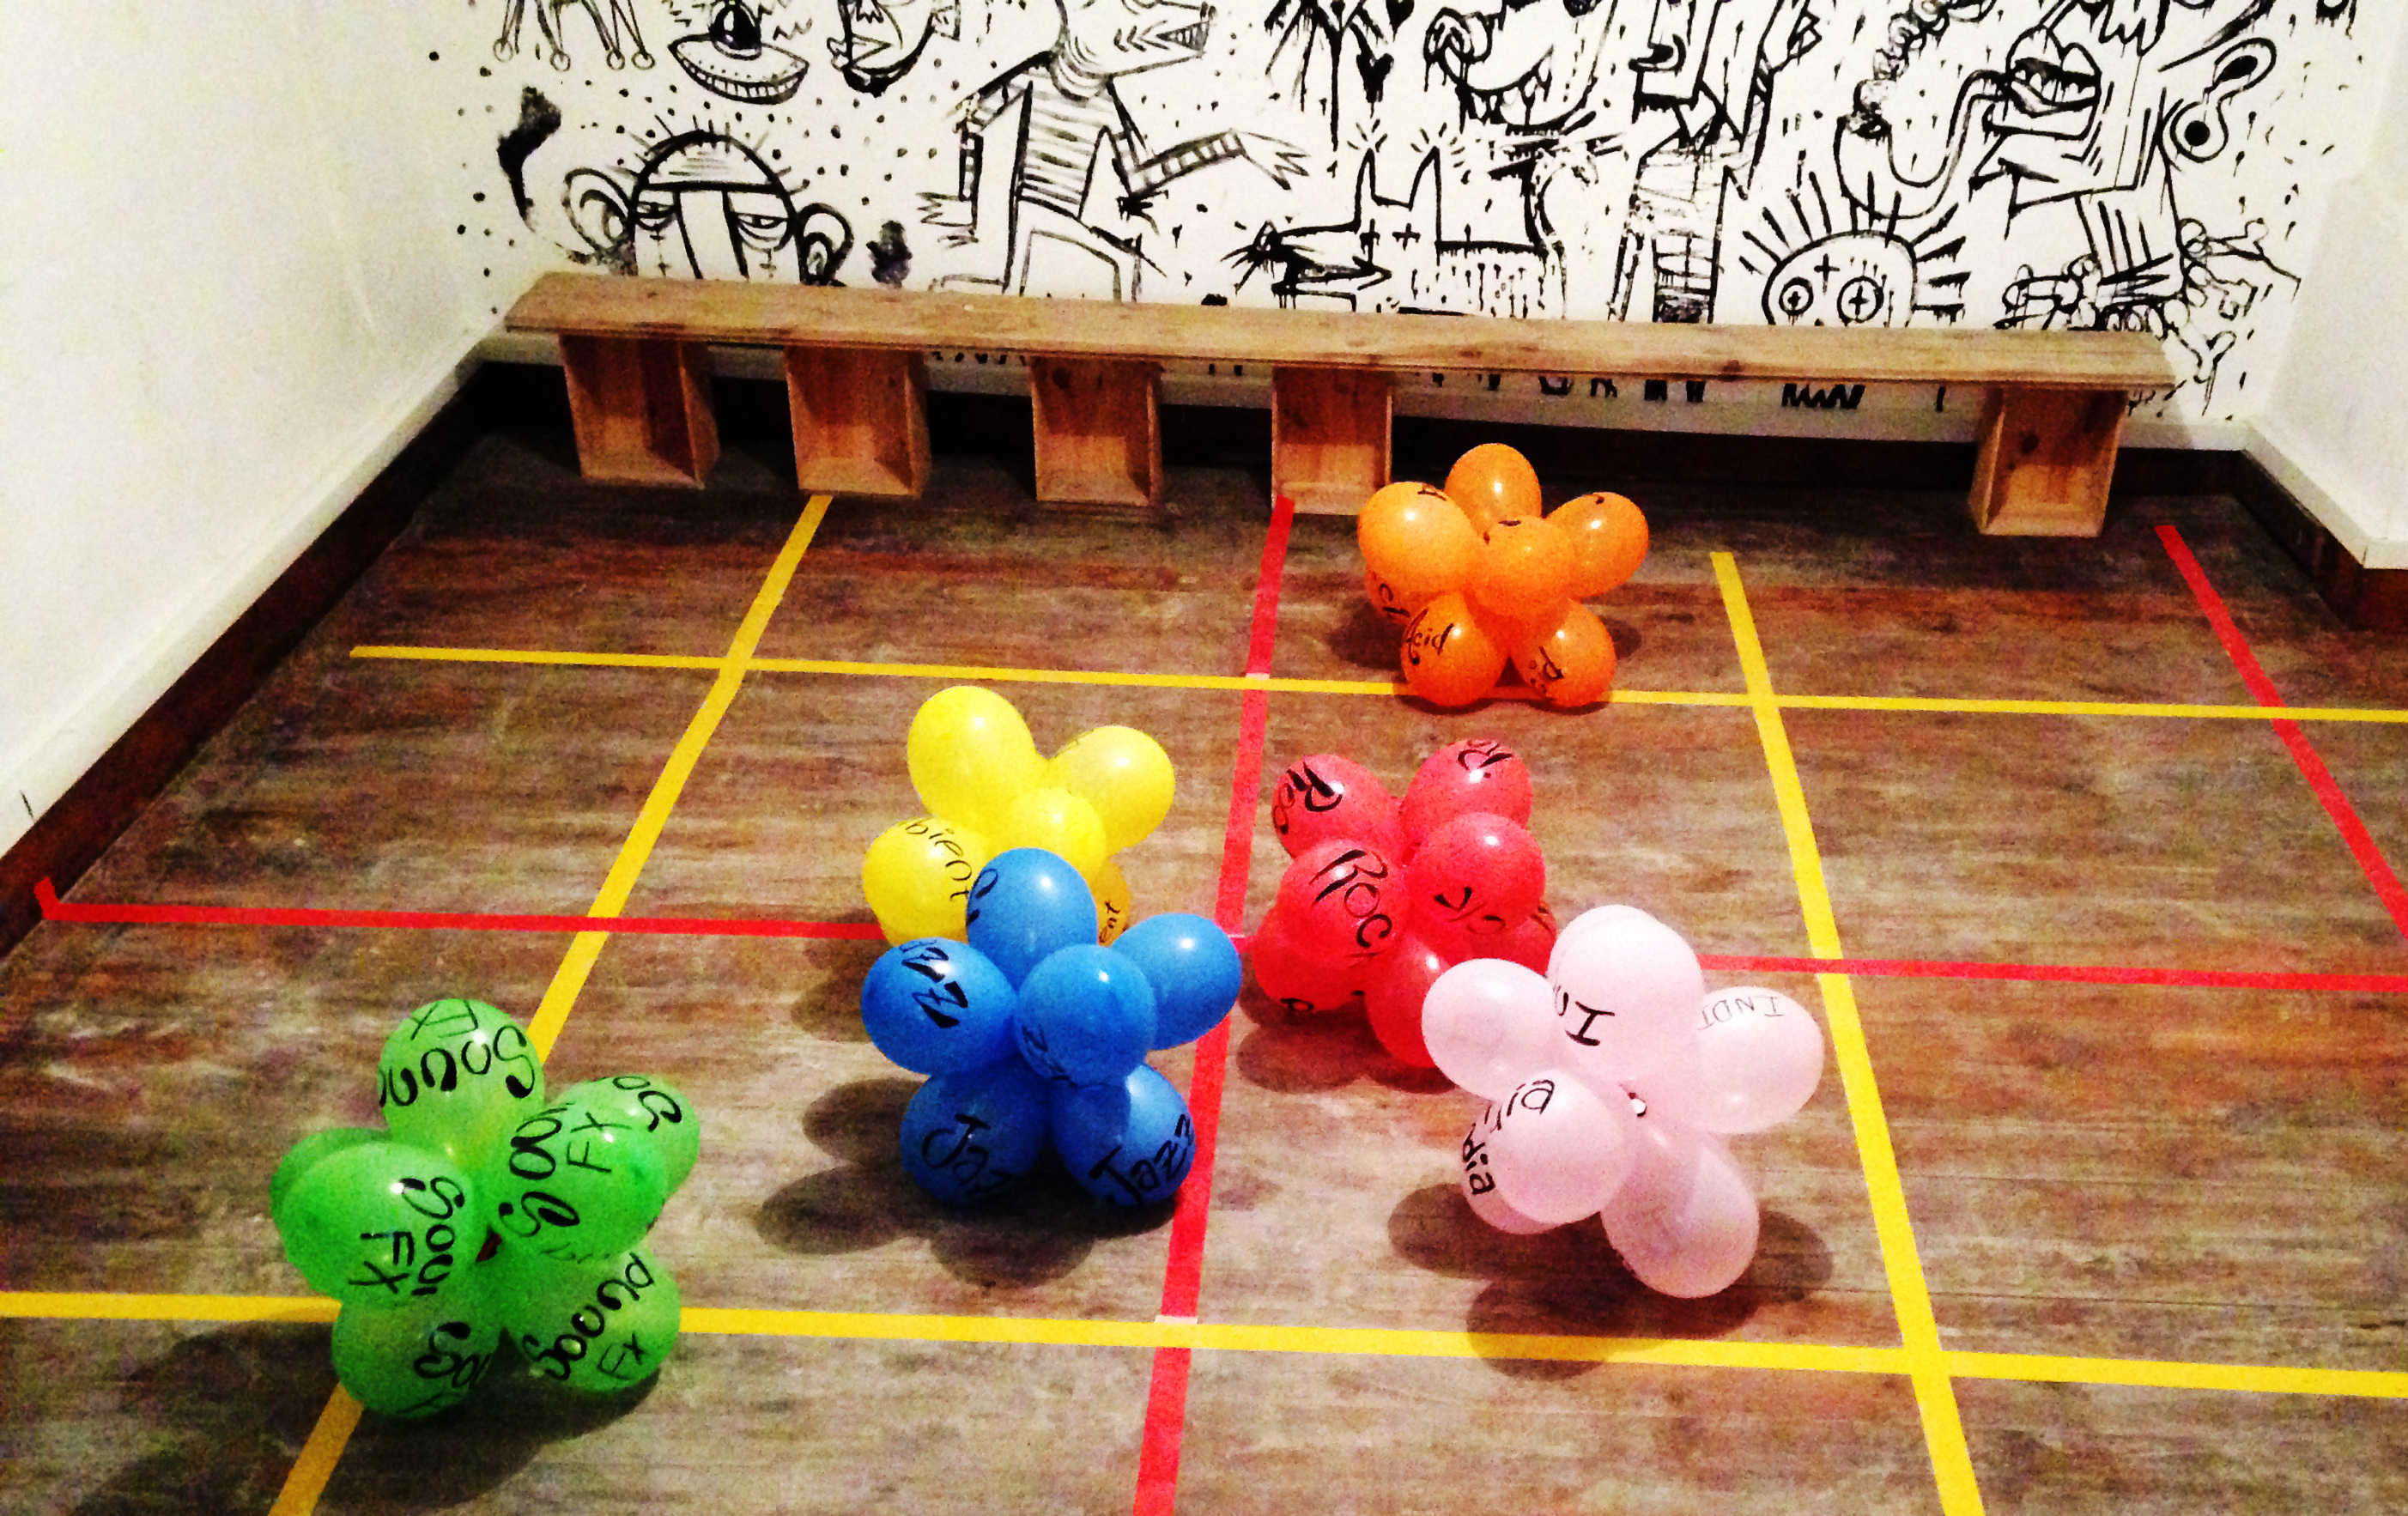
\includegraphics[width=\linewidth]{balloons}
	\caption{Balloon bundles on the dance floor (pilot experiment)}\label{fig:balloons}
\end{figure}

Figure \ref{fig:balloons} shows the system's elements on the dance floor.
It consists of few balloon bundles, each marked with the name of a specific musical style (e.g.\ rock, jazz, Indian music).
A corresponding Bluetooth beacon is installed inside each of these bundles.
After downloading and installing the Android application, strolling between the balloon bundles affects the music in one's headphones according to the relative distance from the bundles, creating a virtual ``sound zone'' around each of them.
In addition, the distance from the center of each sound zone may affect the music in several different ways; for example, by controlling the volume, filter, and granularity of the sound zone.
Lastly, participants can move the balloon bundles freely, thereby dynamically changing the structure of the music in the virtual space and making it socially interactive.

Figure \ref{fig:sys:participant_view} shows an overhead view of a possible scenario of participants using the system in a party.

\begin{figure}[!htb]
	\centering
	\def\svgwidth{0.9\textwidth}
	\input{graphics/system_participant_view.pdf_tex}
	\caption{The figure shows schematically two participants, $A$ and $B$, dancing around three Bluetooth beacons, corresponding to the rock, jazz, and Indian music sound zones. Participant $A$ hears rock music and participant $B$ hears a mixture between the jazz and the Indian music sound zones, which are rhythmically and harmonically synchronized with each other. A video demonstration of a similar scenario can be found at \href{http://youtu.be/2kJoeD2iWBA}{youtu.be/2kJoeD2iWBA}.}\label{fig:sys:participant_view}
\end{figure}

\subsection{The BBRIP system}

The implementation of the system can be described by two different processes: the development of the BBRIP system (described in this section) and the Android application that wraps it and is responsible for the audio processing (see section \ref{sceneplayer_plus}).

The BBRIP system is my intent to develop an indoor positioning system that satisfies the relatively simple requirements of the research as presented in section \ref{methods:ips}.

My implementation of the system is based on a specific element in the Bluetooth protocol -- the Received Signal Strength Indicator (RSSI) ({\cite{bray12}).
Each Bluetooth enabled device calculate RSSI values during Bluetooth discovery, when it finds a new device and before establishing connection.

\begin{figure}[!htb]
	\centering
	\def\svgwidth{\columnwidth}
  	\input{graphics/bbrip.pdf_tex}
	\caption{The BBRIP system}\label{fig:bbrip}
\end{figure}

As shown in figure \ref{fig:bbrip}, the BBRIP system continuously searches for Bluetooth devices.
When a new device is found, the RSSI value is extracted and sent forward for processing.
From the first discovery in the Bluetooth discovery cycle, the system keeps checking if the time since the last discovery exceedes a pre-defined timeout. If so, it terminates the discovery.
This termination is important, because naturally a device can only be discovered once in each Bluetooth discovery cycle, and long periods of time without new discoveries indicates that all of the nearby devices are already found.
Lastly, when the system sees that there is no Bluetooth discovery running (because of termination or simply the end of the discovery cycle), it starts a new one immediately.

Although the RSSI values extracted by the BBRIP system are not very precise as a distance estimation, I have found them sufficient in order to classify the distance between participants and beacons into useful ranges. In other words, RSSI values gives great indication if a participant stands close to specific beacon (around 1 meter), in an intermediate range (2 to 3 meters), or in a greater distance.

\subsection{ScenePlayer Plus}\label{sceneplayer_plus}

The development of the Android application moved through different development stages.

First, I developed an application that didn't use ``libpd'' at all (see section \ref{methods:libpd}).
In this early stage the only effect of approaching or leaving a beacon was a change in the volume.
In addition, the limited sophistication of the built-in audio library made fading in and out from the sound zones very inflexible.

After finding the weakness of using the built-in audio library of the Android application programming interface, I decided to implement the system using ``libpd''.
Although this implementation worked, it made a very tight coupling between the system development in the Android environment and the audio processing development in Pd.
Overall, this development phase was sufficient, but in order to allow other musicians and developers to use the system I started to look for a more open architecture, that maintains a loosely coupled connection between the Android application and the Pd patch that drives the audio.

The last phase in the system development was to implement the BBRIP system into the open source Android application ``ScenePlayer''\footnote{ScenePlayer: \href{http://play.google.com/store/apps/details?id=org.puredata.android.scenes}{play.google.com/store/apps/details?id=org.puredata.android.scenes}.}, an Android port for the RjDj application mentioned in section \ref{rjdj}, and release it again as ``ScenePlayer Plus''\footnote{ScenePlayer Plus: \href{http://play.google.com/store/apps/details?id=com.nagasaki45.sceneplayerplus}{play.google.com/store/apps/details?id=com.nagasaki45.sceneplayerplus}.}.
The application exposes the Bluetooth RSSI values to the Pd patch as another sensor of the mobile device (e.g.\ accelerometer, compass and touchscreen).

\section{Experiment I}

In order to evaluate the social effects of the system's usage I decided to conduct controlled experiments.
For the sake of evaluating the system in its most natural designation, the context of the experiments was selected to be a silent disco party.
The experiments' main goal is to answer the research question: \emph{does the system enhance social interaction between participants in an interactive silent disco party?}
In addition, an implied hypothesis is that participating in a party using the system strengthens the social relationships between participants even beyond the scope of the party.

Assessing the social interaction between participants was done using two main methods: self-reported information that the participants entered in surveys before, during, and after each experiment, and with objective measurements such as participants positioning tracking and their interaction with system components. 

The following sections present the pilot experiment that has been done, the motivation for an experiment of a larger scope, and a detailed explanation of the experimental design.

\subsection{Methods}

\begin{figure}[!htb]
	\centering
	\def\svgwidth{0.95\columnwidth}
  	\input{graphics/pilot_design.pdf_tex}
	\caption{Pilot experiment design}\label{fig:pilot}
\end{figure}

Eighteen volunteers were invited to participate in an interactive silent disco party.
Each participant installed the Android application on his or her phone and filled pre/post party surveys that included questions regarding their musical background and preferences as well as system evaluation feedback.
The party consisted of four alternating interactive/control blocks of duration 5:40 minutes each (see figure \ref{fig:pilot}).
The participants were randomly assigned to two groups: $A$ and $B$, comprising the interactive and control blocks respectively\footnote{Group $A$ (interactive first) consisted of 8 participants (4 females and 4 males) with mean age of 36.7 (s.d=12.3); group $B$ (control first) consisted of 10 participants (3 females and 7 males) with mean age of 29.6 (s.d=10.2). Participants had a diverse musical background with 4.7 mean years of musical training (s.d=5.2).}.
They were informed that the experiment consists of interactive and control segments, however, they were not informed about the exact schedule and timing of the blocks or the group assignments.
Both groups started the experiment together.
In the interactive blocks, the application generated music as described in section \ref{systemdescription}, whereas in the control blocks the participants heard recorded non-interactive music created in advance using the musical material of the interactive system\footnote{The control block music composed by Noam Elron (\href{http://www.noamelron.com}{www.noamelron.com}).}.

Interaction with the system's components was assessed by counting the number of Bluetooth device discoveries made by each participant's phone during both the interactive and the control blocks.
In order to eliminate edge effects, we analyzed only the two middle blocks of the experiment.

\subsection{Results}

\begin{figure}[!htb]
\minipage{0.49\textwidth}
	\def\svgwidth{0.95\columnwidth}
  	\input{graphics/changing_location_in_space.pdf_tex}
	\caption{Changing location in space}\label{fig:location}
\endminipage\hfill
\minipage{0.49\textwidth}
	\def\svgwidth{0.95\columnwidth}
	\input{graphics/dancing_with_known_people.pdf_tex}
	\caption{Dancing with known people}\label{fig:known}
\endminipage\hfill
\end{figure}

In the post-party survey, participants self-reported significantly higher levels of movement (paired t-test, $t(15)=3.9$, $p<0.01$) using the system, compared with their behavior at other parties as reported in the pre-party survey.
Figure \ref{fig:location} shows that there was a significant difference (unpaired t-test, $t(33)=6.2$, $p<0.01$) in the mean response to these questions (at a scale of 1-3).

In order to objectively assess if participants moved more in space, we measured the counting of Bluetooth discoveries made by the applications' BBRIP system.
The results show slightly higher counts (paired t-test, $t(16)=1.7$, $p=0.06$, n.s) during the interactive blocks of the party compared with the control blocks. This suggests that the interactive components of the system facilitated greater participant movement in space, thereby offering more frequent opportunities for social interactions.
Indeed, in the post-party survey participants reported that they danced significantly less with people that they knew in advance, compared with their usual behavior (paired t-test, $t(14)=-2.5$, $p=0.01$).
Figure \ref{fig:known} shows that there was also a significant difference in the mean response to these questions in the pre/post surveys.
Overall, participants showed a slightly stronger tendency (paired t-test, $t(16)=1.46$ ,$p=0.08$, n.s) to participate in an interactive party in the post-party survey, compared with their answer to identical questions in the pre survey.

The preliminary results already demonstrate the potential for audio-only augmented reality to significantly enrich the experience of music consumption and its attendant social interaction.
This can be validated in a controlled experiment using both direct reports of subject and indirect objective measurements.

\subsubsection{Video analysis}

\begin{figure}[!htb]
    \centering
    \includegraphics[width=0.8\textwidth]{plots/pilot-familiarity_correlation_maps.pdf}
    \caption{Maps of social familiarity (on the left) and correlated movement on the dance floor (on the right)}\label{plot:pilot-familiarity_correlation_maps}
\end{figure}

The whole experiment was captured with video from above the dance floor. Later, this video was used to track the positioning of the participants and to generate positioning tables.

Analyzing this data, we didn't find significant difference between the position and movement patterns in the interactive and control blocks.
However position was indicative to the social relations between participants.
We asked participants for their social relationships to other participants and compared the resulted map with a map of positioning correlation between every two participants\footnote{This data was measured along the Y axis only, which was much more indicative then the X axis due to the fact that the length of the dance floor (the Y axis) was 10 meters when the width of it was only 2.5 meters.}.
We used Monte Carlo reshuffling to check how similar those two maps are and we found the matrices are unusually similar (p < 0.001).

To conclude, these results demonstrate how close social connection between participants can also be found in video analysis data.
This encouraging results drove much of the methods to analyze the social behavior in experiment 2.

\section{Experiment II}

\todo[inline]{Rewrite, changing future references to past}

\subsection{Filling the gap}

Although the pilot experiment results already support the hypothesis that the system usage enhances the social interaction between participants, it does not shed a light on the following points:

\begin{itemize}
	\item It does not distinguish between participants that knew one another in advance.
	\item It does not show that the social effects of the system extends beyond the scope of the system usage.
\end{itemize}

The following experiment design is intended to clear up those points.
First, by assuming that participants in a party are pre-partitioned into groups of friends, and thereby a major effort will be made to gain better understanding of the behavior of those groups as a whole and the behavior of each participant as a member of a group.
Second, by using a control group that will not experience the interactive part of the system at all, and will be socially compared to the experiment group before and after the experiment.

\subsection{Methods}\label{methods:evaluation}

\subsubsection{Participants}

Thirty undergraduate and graduate-level students from the Music Department of Bar-Ilan university will participate in the experiment.
Their participation will rely on voluntary will.

\subsubsection{Measurements}

The above research question will be fragmented into the following operational definitions and measurements\footnote{Complete version of each of the surveys below can be found in the appendix.}:
\begin{enumerate}
	\item \label{measure:partitioning} Participants will report their familiarity with other participants using a survey based on the experimental ordinal number.
	\item \label{measure:disperse} Using the above partitioning to groups of friends we can define the \definition{momentary center} of each group as the average positioning of its participants on the two-dimensional plain of the dance floor (measured by video tracking as explained in section \ref{aparatus}).
	In addition, we can define the \definition{momentary disperse} of each group as

	\begin{equation*}
		\sum_{i=1}^n \frac{\sqrt{(x_i - \mu_x)^2 + (y_i - \mu_y)^2}}{n}
	\end{equation*}

	where $(x_i, y_i)$ are the positioning of the group members on the dance floor and $(\mu_x, \mu_y)$ is their \definition{momentary center}.
	Using the above definitions interaction between the members of one group with other participants will be evaluated by the disperse of the groups, when high disperse values indicate higher interactivity.
	\item \label{measure:groups} Using the above definitions, we can define \definition{momentary group disperse} as the dispersal of momentary centers themselves on the dance floor.
	In this regard, low momentary group dispersal values indicate higher interactivity.
	\item \label{measure:audio} The audio volume inside the experiment room will be used as an objective measure of the social state of the group (e.g indicating the ``speaking'' level between participants).
	\item \label{measure:survey:social} Participants will fill out a social interaction survey.
	The survey will be used to asses interaction between participants by estimating social cohesiveness within in-group and out-group of each participant.
\end{enumerate}
In addition to measurements intended to assess the main research question, the following operational definitions and measurements will be used in order to assess interaction with and satisfaction from the system.
\begin{enumerate}[resume]
	\item \label{measure:system} We will define \definition{momentary participant-system interaction} as the momentary distance of each participant from the closest Bluetooth beacon.
	Using the above definition high level of interaction of participant with the system will be indicated by low values of momentary participant-system interaction.
	\item \label{measure:survey:usability} Participants will fill system satisfaction survey, based on the System Usability Scale (\cite{brooke96}).
\end{enumerate}
Lastly, the following measurement will be used in order to eliminate possible differences between research groups and to allow future research based on the retrieved data.
\begin{enumerate}[resume]
	\item \label{measure:survey:musical} Participants will fill musical background survey, based on the Emmanuel College Music Background Questionnaire, basic version (\cite{web:zhao12}).
\end{enumerate}

\subsubsection{Apparatus}\label{aparatus}

In order to measure momentary dispersal and group dispersal as defined in measurements \ref{measure:disperse} and \ref{measure:groups} I will capture the experiment with a video camera from above the dance floor.
Tracking the positioning of the participants will be done semi-manually using software aids to record the manual tracking of participants, one at a time, using the computer mouse.
The results will be then processed using computational programming to conclude insights from the data.

Tracking data required in order to compute momentary participant-system interaction, as described in measurement \ref{measure:system}, will be derived the same way, by manually tracking each one of the system components in the video.

Audio volume (measurement \ref{measure:audio}) will be captured by a microphone and analyzed afterwards.

\subsubsection{Procedure}

Participants will be randomly allocated into two groups, group $A$ and group $B$\@.
Each group will participate in the experiment in different week, but on the same day of the week and same hour.

\begin{figure}[!htb]
	\centering
	\def\svgwidth{0.9\textwidth}
  	\input{graphics/procedure.pdf_tex}
	\caption{Experiment design}\label{fig:experiment}
\end{figure}

Participants will first fill a musical background survey (measurement \ref{measure:survey:musical}) and a participants familiarity survey (measurement \ref{measure:partitioning}), followed by three \definition{experiment blocks}, followed by a system usability survey (measurement \ref{measure:survey:usability}) as shown in figure \ref{fig:experiment}.
After filling out the system usability survey the participants will experience another experiment block\footnote{The existence of the last experiment block is there in order to allow the control group to experience the interactive component of the system, eliminating possible frustration and feeling of discrimination between the groups.}.
In each experiment block the participants will listen to music in their headphones, using their Android device and pre-installed application, and will interact with other participants and system components in the `silent disco' party.
Meanwhile, during each experiment block, measurements \ref{measure:disperse}, \ref{measure:groups}, \ref{measure:audio} and \ref{measure:system} will be collected.
Before each experiment block and after the last block each participant will fill the social interaction survey (measurement \ref{measure:survey:social}).

Each experiment block could be of one of the following types:
\begin{description}
	\item[Interactive:] In which the music generated by the Android application behaves as described in section \ref{systemdescription}.
	\item[Control:] In which the music generated by the Android application is pre-composed and based on the same musical materials as of the interactive system.
\end{description}

Participants of group $A$ will hear the experiment blocks: Control $\rightarrow$ Control $\rightarrow$ Control $\rightarrow$ Interactive. Whereas participants of group $B$ will hear the experiment blocks: Control $\rightarrow$ Interactive $\rightarrow$ Control $\rightarrow$ Interactive.

The procedure described above presents several advantages in assessing the main research question:
First, the comparison between the effects of interactive and control blocks could be done as a between-group evaluation in relation to the second experiment block of each group.
Second, comparison between interactive and control blocks effects could also assessed as a withing-group evaluation between the first and the second, as well as the second and third blocks of group $A$, using group $B$ as a reference.
Lastly, effects on the social interaction beyond the scope of the interactive blocks will be assessed as a within-group evaluation between the first and the third blocks of group $A$, using group $B$ as a reference.

\subsection{Results}

\subsubsection{System satisfaction surveys}

\begin{figure}[!htb]
    \centering
    \includegraphics[width=0.6\textwidth]{plots/usability-sus_scores.pdf}
    \caption{Mean system satisfaction scores for the control and interactive groups}\label{plot:usability-sus_scores}
\end{figure}

\begin{figure}[!htb]
    \centering
    \includegraphics[width=\textwidth]{plots/usability-per_question_statistics.pdf}
    \caption{System satisfaction questionnaire results. Bars indicates the mean response of single questions (questions are listed to the right).}\label{plot:usability-per_question_statistics}
\end{figure}

We used a system satisfaction survey at the end of the experimental session for each of the groups in order to evaluate the engagement of the participants with the system. The survey was based on the standard system usability scale (SUS) survey (\cite{brooke96}) with minor modifications. The SUS survey contain 10 question, 5 of them positive (a larger number indicates larger satisfaction) and 5 of them negative (a larger number indicates smaller satisfaction). We used a score which combines positive and negative questions as suggested by Brook (\cite*{brooke96}). We found that overall system satisfaction score is larger in the interactive group (interactive: 67.3 (3); control: 45.2 (6.9); unpaired t-test, t(21) = 2.81, p \textless{} 0.01).

This effect was not limited to a single question. In fact, four of the ten questions showed significantly higher satisfaction response in the interactive group as indicated by a separated one-tailed t-test (p \textless{} 0.05). All questions but two showed some tendency (p \textless{} 0.1), and the remaining two questions (extended learning in question 10 and technician aid in question 4) are expected to be less relevant to this system. These results are summarized in figure \ref{plot:usability-per_question_statistics}.
These results consistently show that subject that used the interactive component of the system were more satisfied than the control group that had similar physical conditions.

\subsubsection{Social interaction surveys}

\begin{figure}[!htb]
    \centering
    \includegraphics[width=\textwidth]{plots/interaction_surveys-question_2.pdf}
    \caption{Mean participants response to social interaction statements; statement 1: ``In the last experiment block I interacted with close friends only''; statement 2: ``In the last experiment block I interacted with participants with them I have no social connection''}\label{plot:interaction_surveys-question_2}
\end{figure}

One of my main hypotheses was that the system will increase social interaction outside the native groups. Namely, subjects that usually interact less with each other will tend to interact more. To assess this hypothesis I have used social interaction survey between each of the experiment sessions.

Surprisingly, the results of the this survey showed a different trend. The left side of figure \ref{plot:interaction_surveys-question_2} shows the mean response (on a scale of 1 to 5) to the statement ``In the last experiment block I interacted with close friends only''. There was no significant main effects and group by session interactions as indicated by 2-way repeated measure ANOVA (group: F(1, 21)=0.094 p=0.762; session: F(2, 42)=0.835 p=0.441; interaction: F(2, 42)=0.548 p=0.582).

Similar results were obtained for the second question in survey, which was ``In the last experiment block I interacted with participants with them I have no social connection''  (group: F(1, 21)=2.062 p=0.166; session: F(2, 42)=1.730 p=0.190; interaction: F(2, 42)=1.730 p=0.190). Note however a small trend which indicates higher tendency to interact outside the native group in the control group, as indicated by a session main effect and significant interaction of group by session in a repeated measure 2 way ANOVA test between session one and two only (session: F(1, 21)=4.495 p=0.046; interaction: F(1, 21)=4.495 p=0.046). Even though that the overall results did not reach significance this indicates an opposite trend to the results in experiment 1. In experiment 1 subject reported that they used to interact more with subject that they are less familiar with, though in this experiment we had no way to dissociate between using the system interactively and non-interactively.

To conclude, subject did not appear to explicitly interact more with subject that are outside their native group, and we can even identify an opposite trend. As we will shortly see this observation is further supported by the implicit measures.

\subsubsection{Social structure}

\begin{figure}[!htb]
    \centering
    \includegraphics[width=0.8\textwidth]{plots/familiarity-clustering_maps.pdf}
    \caption{Maps of social familiarity between participants where darker colors means low familiarity and lighter colors means high familiarity. The maps on the left are for the control group and on the right for the interactive group. From top to bottom, maps represent the original maps, socially clustered maps using K-means algorithm and socially clustered maps using mean-shift algorithm}\label{plot:familiarity-clustering_maps}
\end{figure}

In experiment 1, participants were recruited using the internet and therefore had varied prior familiarity with each other. This created a strong grouping into social clusters that was also apparent in their positioning in space as indicated by our video tracking analysis (see figure \ref{plot:pilot-familiarity_correlation_maps}). Based on this encouraging results we specifically asked subject to fill a social familiarity survey at the beginning of the experiment. Each subject had to rank its class pears on a scale of 1 to 5 according to social familiarity (see methods). Note that the second experiment group is much more homogeneous since unlike experiment 1 all participants have prior familiarity, since they all study together.

Figure \ref{plot:familiarity-clustering_maps} first row shows pre-clustered social matrices, where the familiarity each participant on the y axis with participants on the x axis is indicated by color. We applied K-means\footnote{K-means: \href{http://scikit-learn.org/stable/modules/clustering.html\#k-means}{scikit-learn.org/stable/modules/clustering.html\#k-means}}.} and mean-shift\footnote{Mean-shift: \href{http://scikit-learn.org/stable/modules/clustering.html\#mean-shift}{scikit-learn.org/stable/modules/clustering.html\#mean-shift}.} clustering algorithms as implemented by the software package Scikit-learn (\cite{scikit-learn}) on these matrices to find out that in this group we did not find clustered social structures. This is indicated by cross cluster similarity outside the main diagonal of the clustered matrices as depicted in the last two rows of figure \ref{plot:familiarity-clustering_maps}.

\subsubsection{Video analysis: Movement}

\begin{figure}[!htb]
    \centering
    \includegraphics[width=0.6\textwidth]{plots/analyze-movement.pdf}
    \caption{Mean speed of participants as movement assessment}\label{plot:analyze-movement}
\end{figure}

Experiment 1 showed that video tracking could be used effectively to gain insights about the social interaction. Based on these encouraging results we used extensively video tracking in experiment 2.

We analyzed the mean speed of each participant during each session. We hypothesis that the interactive system will facilitate movement among the users. However, we found an opposite trend, where in fact, during the second session the participants of the interactive group tend to move significantly less compared with the control group. This trend persist and even increase in the last session of the experiment. These evidences are indicated by a significant interaction of group by session in a repeated measure 2 way ANOVA test (group: F(1, 21)=3.311 p=0.083; session: F(2, 42)=0.579 p=0.455; interaction: F(2, 42)=7.318 p=0.013). Note however, that in the first session, there was no significant difference between the groups ((interactive: 0.269 (0.048); control: 0.258 (0.035); two-sided unpaired t-test, t(21) = -0.18, p = 0.22).

\subsubsection{Video analysis: Interaction with system components}

\begin{figure}[!htb]
    \centering
    \includegraphics[width=\textwidth]{plots/annotations-clustering_example.pdf}
    \caption{Locations of participants and beacons in space for two typical point in time. Blue dots indicates the participants locations; green indicates beacons; red indicate the bench area; yellow annotate clusters of participants and beacons.}\label{plot:annotations-clustering_example}
\end{figure}

\begin{figure}[!htb]
    \centering
    \includegraphics[width=\textwidth]{plots/annotations-correlated_movement_example.pdf}
    \caption{A correlated movement of two participants holding one of the beacons. As we can clearly see this participants move coordinated through a time epoche of 9 seconds.}\label{plot:annotations-correlated_movement_example}
\end{figure}

Animated renditions of the participants movement can be viewed in my site\footnote{Animated movement of participants: \href{http://tomgurion.blogspot.com/2014/10/participants-movement-tracking-videos.html}{tomgurion.blogspot.com/2014/10/participants-movement-tracking-videos.html}.}. Figure \ref{plot:annotations-clustering_example} show a screenshot of one point in time extracted from session 2, for each group. These results show that participants of the interactive group tend to cluster around the interactive components of the system in small groups.

Additional phenomena found in the in video animations is correlate movement of participant as can be seen in the list of consequence screenshots in figure \ref{plot:annotations-correlated_movement_example}.

\begin{figure}[!htb]
    \centering
    \includegraphics[width=0.6\textwidth]{plots/analyze-expectancy_of_participants_close_to_a_beacon.pdf}
    \caption{Expectancy for the number of participants in a 1 meter radius around a beacon}\label{plot:analyze-expectancy_of_participants_close_to_a_beacon}
\end{figure}

These observations are also evident in our statistical analysis. We’ve count the mean number of participants near (less than 1 meters) each beacon over the frames of the video a beacon. Beacons that had no participants around them were excluded from the calculation. As expected from the fact that groups did not differ in the initial procedure in the first  session, there was no significant difference between the group in this session as indicated by a two-sided unpaired t-test (interactive: 1.78 (0.071); control: 1.64 (0.20); t(10) = -0.57, p = 0.15). However the interactive group showed a larger tendency to crowd around the beacons as indicated by a significant group effect in a repeated measure 2 way ANOVA test (F(1, 9)=9.974 p=0.012). This is consistent with the explicit results of the system satisfaction that show that participants were more satisfied and therefore probably more engaged with the system.

\subsubsection{Video analysis: Clustering}

\begin{figure}[!htb]
    \centering
    \includegraphics[width=\textwidth]{plots/analyze-clustering_scores.pdf}
    \caption{Clustering scores. Algorithm score is the mean distance of participants from their momentary cluster centroid. Social score is the mean of the social familiarity of participants (as reported by him/her in the familiarity survey) with any other participant in the same cluster.}\label{plot:analyze-clustering_scores}
\end{figure}

I have used the mean-shift algorithm, as implemented by the software package Scikit-learn (\cite{scikit-learn}), to cluster participants into groups based on their positioning in space. For each frame in the video the algorithm created varied number of participants clusters. These clusters have been used to get the following per participant scores:

\begin{description}
    \item[Algorithm score:] That is the distance of the participant from his cluster centroid. Hence lower scores indicates higher in-cluster interaction.
    \item[Social score:] That is the mean of the social familiarity of the participant (as reported by him/her in the familiarity survey) with any other participant in the same cluster.
\end{description}

The final algorithm / social score for each participant is his / her average score over the frame of the whole session.

As shown in figure \ref{plot:analyze-clustering_scores} left plot, there was a significant difference between the second session of the interactive and the control group in the algorithm score as indicated by a significant group and interaction of group by session effects in a repeated measure 2 way ANOVA test (group: F(1, 21)=6.987 p=0.015; interaction: F(2, 42)=8.202 p=0.001). Note however, that in the first session, there was no significant difference between the groups (interactive: 0.940 (0.044); control: 0.866 (0.053); two-sided unpaired t-test, t(21) = -1.017, p=0.080).

These results indicating that using the interactive system participants tend to cluster in more dense clusters, confirming the observed clustering from the video animations. This effect persist over the last block, but with less significance.

Similarly to the results from the interactive surveys, figure \ref{plot:analyze-clustering_scores} right plot shows a non-significant group by session effect over the clusters social scores; whereas in the interactive group participants tend to cluster with others that are socially close to them, the participants of the control group tend to cluster with participants that are far from them socially on the social map (repeated measure 2 way ANOVA; interaction: F(2, 42)=2.032 p=0.144).

\section{Discussion}

\todo[inline]{Write discussion section}

\begin{appendices}

\section[Musical background survey]{Musical background survey\\
	{\normalsize based on the Emmanuel College Music Background Questionnaire, basic version}}

Please first provide your basic information.

\begin{enumerate}
	\item Name: \myunderline
	\item Gender: Male / Female
	\item Age: \myunderline
	\item E-mail: \myunderline
\end{enumerate}
Please answer the following questions to the best of your knowledge.
\begin{enumerate}[resume]

	\item Please rate your overall interest in music according to the following scale

	\begin{tabular}{c c c c c}
		Not interested & & Neutral & & Very interested \\
		1 & 2 & 3 & 4 & 5 \\
	\end{tabular}

	\item Please rate your overall musical ability according to the following scale

	\begin{tabular}{c c c c c}
		Poor & & Average & & Excellent \\
		1 & 2 & 3 & 4 & 5 \\
	\end{tabular}

	\item How many hours per week do you spend listening to music?

	\myunderline

	\item What genre(s) do you listen to most? (check all that apply)

	\begin{tabular}{l l}
		{[{ \ }]} & Classical \\
		{[{ \ }]} & Country \\
		{[{ \ }]} & Jazz \\
		{[{ \ }]} & Rock \\
		{[{ \ }]} & Pop \\
		{[{ \ }]} & Non-western \\
		{[{ \ }]} & Other: (please specify) \myunderline \\
	\end{tabular}

	\item Most of the time, when you listen to music, you are

	\begin{tabular}{l l}
		( \ ) & not focused on the music, attending to a different task \\
		( \ ) & passively listening \\
		( \ ) & highly aware of musical nuances such as key changes, harmonies, etc. \\
		( \ ) & actively engaged (sing along, tap the beat, etc.) \\
	\end{tabular}

	\item About how many hours of musical activity do you engage in each week currently? (e.g.\ practice, performance)

	\myunderline

	\item \label{appendix:music:ensamble}Have you ever participated in a musical ensemble?

	\begin{tabular}{l l}
		( \ ) No \\
		( \ ) Yes, instrumental ensemble \\
		( \ ) Yes, vocal ensemble \\
		( \ ) Yes, both instrumental and vocal \\
	\end{tabular}

	\item If you answered YES to question \ref{appendix:music:ensamble}, please indicate how many years you have participated in the music ensemble

	\myunderline \ years

	\item Please list any instrument(s) that you play (including voice) and the years you play each of them, beginning with your primary instrument:

	\begin{tabular}{c c}
		Instrument &  Years playing \\
		\myunderline & \myunderline \\
		\myunderline & \myunderline \\
		\myunderline & \myunderline \\
		\myunderline & \myunderline \\
	\end{tabular}
	
	\item \label{appendix:music:before_break}Have you ever had any formal training in music? (If you are a self-taught musician, please also answer YES)

	\begin{tabular}{l l}
		( \ ) & YES, I had a formal training in music \\
		( \ ) & YES, I consider myself a self-taught musician \\
		( \ ) & NO \\
	\end{tabular}

\end{enumerate}
Please continue this form if you answered YES to question \ref{appendix:music:before_break}, otherwise please go directly to question \ref{appendix:music:after_break}.
\begin{enumerate}[resume]

	\item What type(s) of music training have you had? (check all that apply)

	\begin{tabular}{l l}
		{[{ \ }]} & private/small group lessons in instrument and/or voice \\
		{[{ \ }]} & institutional training \\
		{[{ \ }]} & University degree in music - list degree: \\
		{[{ \ }]} & self-taught \\
		{[{ \ }]} & other (please specify): \myunderline \\
	\end{tabular}

 	\item At what age did you begin to study music?

 	\myunderline

 	\item How long did your formal music training last?

 	\myunderline \ years
 	\item How long has it been since you last participated in formal music lessons?

	\begin{tabular}{l l}
		( \ ) & Currently have one \\
		( \ ) & Or \myunderline \ years \\
	\end{tabular}

	\item \label{appendix:music:after_break}If there is anything else that you feel is interesting or important about your musical background, please comment below:

	\rule{4.5in}{.5pt} \\
	\rule{4.5in}{.5pt} \\
	\rule{4.5in}{.5pt} \\
	\rule{4.5in}{.5pt}.

\end{enumerate}

\section{Social interaction survey}

\begin{tabularx}{\textwidth}{p{2in} | Y Y Y Y Y }
	& Strongly disagree & & & & Strongly agree \\
	\hline
	In the last experiment block I interacted with people I knew before the experiment & 1 & 2 & 3 & 4 & 5 \\
	\hline
	In the last experiment block I interacted with people I did not know before the experiment & 1 & 2 & 3 & 4 & 5 \\
\end{tabularx}

\section[System satisfaction survey]{System satisfaction survey\\
	{\normalsize based on the System Usability Scale}}

\begin{tabularx}{\textwidth}{p{2in} | Y Y Y Y Y }
	& Strongly disagree & & & & Strongly agree \\
	\hline
	I think that I would like to use this system frequently & 1 & 2 & 3 & 4 & 5 \\
	\hline
	I found the system unnecessarily complex & 1 & 2 & 3 & 4 & 5 \\
	\hline
	I thought the system was easy to use & 1 & 2 & 3 & 4 & 5 \\
	\hline
	I think that I would need the support of a technical person to be able to use this system & 1 & 2 & 3 & 4 & 5 \\
	\hline
	I found the various functions in this system were well integrated & 1 & 2 & 3 & 4 & 5 \\
	\hline
	I thought there was too much inconsistency in this system & 1 & 2 & 3 & 4 & 5 \\
	\hline
	I would imagine that most people would learn to use this system very quickly & 1 & 2 & 3 & 4 & 5 \\
	\hline
	I found the system very cumbersome to use & 1 & 2 & 3 & 4 & 5 \\
	\hline
	I felt very confident using the system & 1 & 2 & 3 & 4 & 5 \\
	\hline
	I needed to learn a lot of things before I could get going with this system & 1 & 2 & 3 & 4 & 5 \\
\end{tabularx}

\end{appendices}

\sloppy  % fixing line breaks in bibliography
\printbibliography[title={Bibliography}]
\end{document}